\begin{flushleft}
	\section{\textcolor{cyan}{Contexte général du projet et cahier de charge}}
	\subsection{\textcolor{green}{Cahier de charge :}}
	Le cahier des charges décrit les différentes tâches à accomplir pour réaliser le système d'irrigation connecté qui collecte des données de capteurs à l'aide d'un Arduino Uno, communique avec un NodeMCU via I2C, envoie les données à un serveur Firebase, affiche les données sur un smartphone sous forme de graphiques et permet de commander une pompe à partir du smartphone.\newline
	
	Collecte de données avec l'Arduino Uno :
	L'Arduino Uno doit être programmé pour collecter les données des capteurs. Les capteurs peuvent être de différents types, tels que des capteurs de température, d'humidité, de pression, de mouvement, etc. Les données collectées doivent être stockées dans la mémoire de l'Arduino Uno ou envoyées directement au NodeMCU via I2C.\newline
	
	Communication I2C de l'Arduino Uno avec le NodeMCU :
	Le NodeMCU doit être configuré en tant que maître I2C et l'Arduino Uno en tant qu'esclave I2C. Les deux doivent être connectés à l'aide des broches SDA et SCL. La communication I2C permettra à l'Arduino Uno d'envoyer les données collectées au NodeMCU.\newline
	
	Envoi des données à un serveur Firebase :
	Le NodeMCU doit être programmé pour se connecter à un serveur Firebase et envoyer les données collectées. Firebase est un service de base de données en temps réel, qui permet de stocker et de synchroniser les données en temps réel entre les appareils. Les données envoyées au serveur Firebase peuvent être stockées dans une base de données en temps réel ou dans un stockage cloud.\newline
	
	Affichage des données dans un smartphone :
	Une application mobile doit être développée pour afficher les données stockées dans la base de données Firebase. L'application doit être capable de se connecter à Firebase et de récupérer les données en temps réel. Les données doivent être affichées sous forme de graphiques pour une meilleure compréhension.\newline
	
	Commande d'une pompe à partir du smartphone :
	L'application mobile doit également permettre de commander une pompe à partir du smartphone. L'application doit envoyer une commande au NodeMCU via Firebase pour allumer ou éteindre la pompe.\newline
	
	En conclusion, pour réaliser ce projet, il faut:\newline
	
	\begin{enumerate}
		\item Programmer l'Arduino Uno pour collecter les données de capteurs et les envoyer au NodeMCU via I2C.
		\item 	Programmer le NodeMCU pour se connecter à Firebase et envoyer les données collectées.
		\item 	Développer une application mobile pour afficher les données en temps réel sous forme de graphiques et commander une pompe à partir du smartphone.
	\end{enumerate}
	\subsection{\textcolor{green}{L'internet des objets}}
	
	\subsubsection{\textcolor{blue}{Définition :}}
	L'Internet des objets (IdO ou IoT en anglais pour Internet of Things) est un concept technologique qui consiste à connecter des objets de la vie quotidienne à Internet, leur permettant ainsi de communiquer et d'échanger des données entre eux et avec les utilisateurs.\newline
	
	Ces objets connectés peuvent être des appareils électroménagers, des montres intelligentes, des capteurs de température, des systèmes de sécurité, des équipements médicaux, des voitures, des éclairages de ville, etc. Ils peuvent être contrôlés, surveillés et interagir avec les utilisateurs via une application mobile ou un site web.\newline
	
	L'Internet des objets permet de collecter et d'analyser des données en temps réel, ce qui peut être utile pour des applications telles que la surveillance de l'environnement, la gestion de l'énergie, la maintenance prédictive, la sécurité, la santé, etc.\newline
	
	Cependant, le développement de l'IdO soulève également des préoccupations liées à la sécurité et à la vie privée, car la collecte de données peut être intrusive si elle n'est pas correctement encadrée.\newline
	\subsubsection{\textcolor{blue}{Les protocoles de communication adoptés par les solutions IoT}}

	Les protocoles de communication adoptés par les solutions IoT (Internet des objets) varient en fonction de plusieurs facteurs tels que la taille et la complexité du réseau, les exigences en matière de bande passante, la consommation d'énergie et la sécurité.\newline
	
	Voici quelques-uns des protocoles de communication couramment utilisés dans les solutions IoT :\newline
	
	\underline{MQTT} (Message Queuing Telemetry Transport) : Il s'agit d'un protocole de messagerie léger et efficace pour la communication entre les appareils IoT et les serveurs. MQTT est conçu pour les connexions à faible bande passante et à latence élevée, ce qui le rend idéal pour les applications IoT.\newline
	
	\underline{CoAP} (Constrained Application Protocol) : Il s'agit d'un protocole de communication Web conçu pour les appareils à ressources limitées. CoAP utilise une approche RESTful (Representational State Transfer) pour la communication entre les appareils et les serveurs.\newline
	
	\underline{BLE}(Bluetooth Low Energy) : Il s'agit d'un protocole sans fil utilisé pour la communication entre les appareils IoT de proximité, tels que les capteurs et les dispositifs portables. BLE est conçu pour une faible consommation d'énergie et une courte portée de transmission.\newline
	
	\underline{Zigbee} : Il s'agit d'un protocole de communication sans fil conçu pour les réseaux à faible consommation d'énergie et à faible débit de données. Zigbee est largement utilisé dans les systèmes de domotique et les applications industrielles.\newline
	
	\underline{LoRaWAN} : Il s'agit d'un protocole de communication sans fil à longue portée conçu pour les applications IoT à grande échelle, telles que les réseaux de capteurs urbains et les réseaux de suivi d'actifs. LoRaWAN utilise une modulation de spectre étalé pour améliorer la portée de transmission et réduire la consommation d'énergie.\newline
	
	 \underline{WiFi} :Le WiFi pour l'IoT utilise les normes WiFi existantes telles que WiFi 802.11b/g/n/ac/ax. Cependant, pour les applications IoT, les fonctionnalités de faible consommation d'énergie, telles que le WiFi Low Energy (WiFi LE), peuvent être utilisées pour réduire la consommation d'énergie lorsqu'un appareil n'est pas en cours d'utilisation.
		\begin{figure}[h]
			\centering
			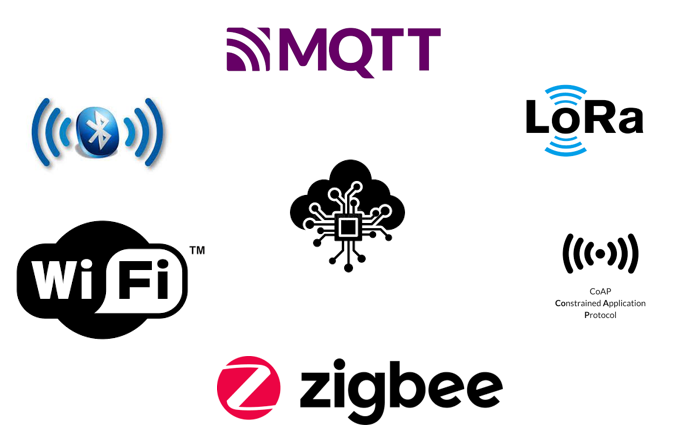
\includegraphics{chapitres/images/Iot-protocol.PNG}
			\caption{protocoles de communication couramment utilisés dans les solutions IoT}
			\label{fig:labelname}
		\end{figure}
	\newpage
	\subsubsection{\textcolor{blue}{Les plateformes matérielles adoptées par les solutions IoT}}
 	\begin{itemize}
 		\item  BeagleBone Black
 		\item  	Raspberry Pi
 		\item  	Intel Edison
 		\item  	ESP32
 		\item  	Mbed board
 		\item  	TI LaunchPad
 		\item  	...
 	\end{itemize}
	
	\subsection{\textcolor{green}{Les technologie de l’internet des objets dans le domaine de l’agriculture de demain}}
	
	\subsubsection{\textcolor{blue}{Drones :}}
	Les drones peuvent avoir plusieurs usages dans l’agriculture qui justifient leurs utilisations. Ils favorisent le rendement, l’inspection rapide des parcelles ou	leurs prises de mesure, l’évaluation instantanée des dégâts de gibiers ou climatiques, la surveillance des parcelles et un épandage facile. Cette arrivée des drones dans le secteur offre un gain de temps considérable, et permet de limiter
	des pertes de production.
	
	L’imagerie aérienne grâce à des capteurs multi spectraux haute résolution permet de connaitre la vitalité des plantations en analysant la quantité de lumière qu’elles absorbent et réfléchissent.
	
	L’agriculteur peut alors prendre les décisions qui s’imposent, en connaissant l’état précis de ses plants, et à un niveau micro-parcellaire.
	Plusieurs caméras sont capables d’effectuer ces relevés, un capteur multi spectral, chargé d’analyser la zone survolée, et un autre capteur qui va quantifier l’intensité de lumière émise par le soleil. Les données de cette caméra peuvent ensuite être traitées via des logiciels adéquats.
	
	Les drones deviennent alors de véritables outils d’aide à la prise de décision, en passant par les ailes volantes, aptes à parcourir de très vastes exploitations agricoles.
	 	
	Le travail des drones pour l’agriculture ne s’arrête pas là, il existe des drones capable de pulvériser de façon extrêmement précise certains engrais et insecticide et des fongicide. L’utilisation de ce système est encore interdite dans quelques pays, mais dans d’autres c’est possible. Ce type de systèmes permet d’effectuer un épandage bien plus précis, adapté et économique, afin de rentrer pleinement dans l’agriculture de précision.
	\begin{figure}[h]
		\centering
		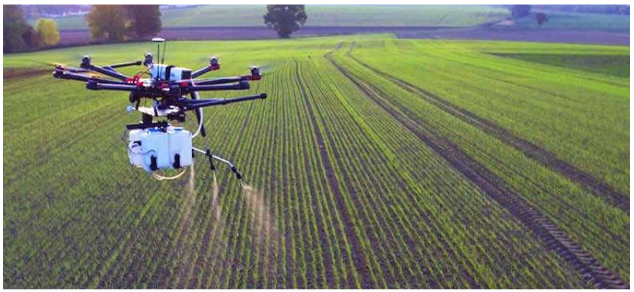
\includegraphics{chapitres/images/Drone.PNG}
		\caption{Des drones agricoles}
		\label{fig:labelname}
	\end{figure}
	
	\subsubsection{\textcolor{blue}{Les robots :}}
		\begin{itemize}
			\item \underline{Agribots} :
		\end{itemize}
	Les agribots sont des petits robots conçus pour accomplir certaines tâches dans le domaine de l’agriculture. Leurs utilisations sont nombreuses : injection d’engrais, arrosage des cultures, désherbage au laser, pulvérisation, récolte de
	légumes, etc.
	 
	Les agribots sont en cours d'intégration dans le monde entier pour aider l'agriculture et améliorer la productivité dans tous les aspects de l'agriculture. Amener les robots dans le domaine agricole peut aider à résoudre de nombreux
	problèmes liés à l'agriculture. A moins que les humains, les machines peuvent fonctionner jour et nuit. Ils peuvent être ajustés pour tolérer la chaleur et l'humidité. Ce processus plus efficace et économique peut également aider à équilibrer les prix sans cesse croissants des produits alimentaires.
	\begin{figure}[h]
		\centering
		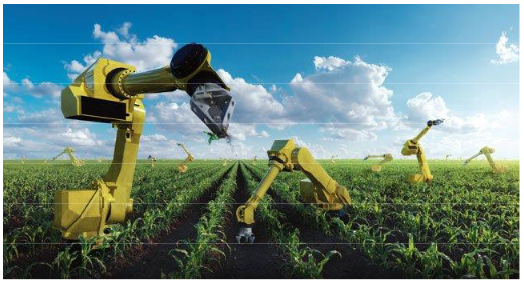
\includegraphics{chapitres/images/Agribots.PNG}
		\caption{Les Agribots}
		\label{fig:labelname}
	\end{figure}
	
	Des systèmes d'ensemencement et de désherbage robotisés peuvent aider les agriculteurs à augmenter les rendements. Dans le but de l'adoption de la robotique agricole à l'avenir est l'investissement croissant du gouvernement.
	
	Cependant, des facteurs empêchent l'adoption de robots dans le secteur agricole, tels que les processus compliqués de l'agriculture et la relation compliquée avec le risque qui pèse sur la communauté agricole. De même, contrairement aux autres industries; l'agriculture est une frontière non conquise pour les robots pour certaines raisons, par exemple, les humains peuvent apprendre la culture mûrie sur place, mais pour les robots, il s'agit d'une tâche mathématique et spatiale complexe nécessitant des capacités telles que 1'intelligence artificielle et l'apprentissage automatique. La machine doit être intelligente pour reconnaître la récolte mûre. Mais si ces tendances se maintiennent au cours des prochaines années, les agriculteurs de toutes formes et de toutes tailles seront de plus en plus à la disposition des agriculteurs et les possibilités de croissance généralisée du marché de la robotique agricole pourraient augmenter considérablement.
		\begin{itemize}
			\item \underline{le robot de binage} :
		\end{itemize}
	La société française est spécialisée depuis 1938 dans les machines
	agricoles pour le travail des sols. Le robot Carré est un robot agricole connecté qui assiste les maraîchers dans leur travail quotidien, de l’entretien des cultures au rapport de synthèse de chaque parcelle, un robot de binage qui effectue un
	désherbage inter-rang et sur le rang, et peut être utilisé pour de nombreux types de cultures maraichères. D'une autonomie de 4h, il est silencieux et dispose d'un système de navigation qui lui permet de s'orienter.
	\begin{figure}[h]
		\centering
		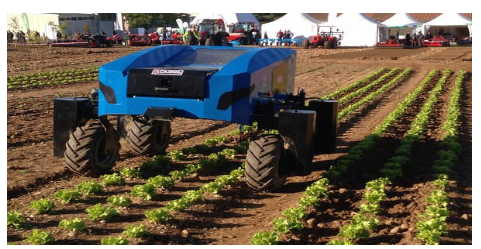
\includegraphics{chapitres/images/robot-binage.PNG}
		\caption{Le robot binage qui cartographie les cultures de salades}
		\label{fig:labelname}
	\end{figure}
	
	Le robot collecte les informations suivantes: température extérieure par capteur,	hygrométrie de l'air par capteur, température et hygrométrie du sol à 10 cm par sonde, enherbement, nombre de pieds au calibre. En plus de l'entretien des
	cultures par binage, ce robot fournit une aide à la décision dans le suivi des cultures par acquisition et traitement d'indicateurs. L’agriculteur reçoit une analyse de ces informations sous forme de tableur Excel ou de cartes, consultables sur Smartphone ou tablette. Le robot peut également être interrogé sur une information en particulier.
		\begin{itemize}
			\item 	\underline{Robot désherber de vignes} :
		\end{itemize}
	
	Ce robot spécialisé pour la tonte est alimenté à l'énergie solaire. La définition des zones à traiter se fait via les coordonnées GPS de la parcelle, avec la possibilité de spécifier des endroits à éviter. Ecologique, il permet de réduire l'usage des désherbants et se pilote simplement avec une application par
	Smartphone.
	\begin{figure}[h]
		\centering
		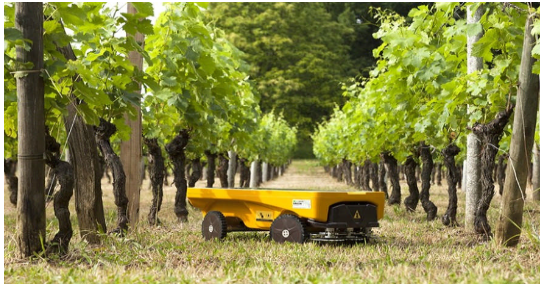
\includegraphics{chapitres/images/Robot-desherber.PNG}
		\caption{Robot désherber de vignes}
		\label{fig:labelname}
	\end{figure}

		\begin{itemize}
			\item \underline{Les tracteurs intelligents sans conducteur} :
		\end{itemize}
	Les tracteurs intelligents sont utilisés pour maximiser les rendements sur des tâches de grande échelle. Des tracteurs connectés peuvent, par exemple, intégrer directement des informations cartographiques pour un apport d’engrais
	sur mesure automatique. Leur équipement GPS permet d’optimiser les chemins au travers des cultures.
	\begin{figure}[h]
		\centering
		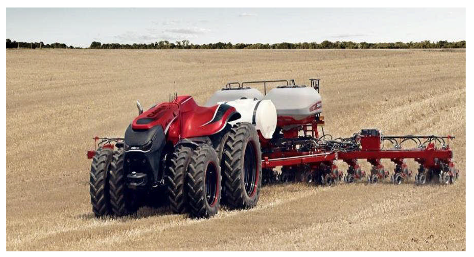
\includegraphics{chapitres/images/tracteurs-intelligents.PNG}
		\caption{Les tracteurs intelligents sans conducteur}
		\label{fig:labelname}
	\end{figure}
	
	
\end{flushleft}
\newpage


